\chapter{Evaluation}
\label{chap:analysis}

The Previous chapter introduced our approach on performance hot-spot detection of configurable software systems. Furthermore, it motivates the choice of the performance extraction tool by evaluating different extraction tools. In this chapter, we discuss the main question of this thesis: \emph{Can we identify performance hot-spots in configurable software systems?} In order to answer this question, we evaluate the applicability of our approach with a case study and answer the following research questions:


\begin{researchq}
	\item How can we define the configuration space of our subject systems?
	\label{rq:config_space}

	\item Are performance hot-spots configuration or workload sensitive?
	\label{rq:sensitivity}

	\item Can we learn performance influence models on method level?
	\label{rq:perf_infl_model}

	\begin{researchq}
		\item How much information can we get by using pair-wise interactions instead of feature-wise??
		\label{rq:interactions}
		\item What influences the learning of performance-influence models?
		\label{rq:learning influence}
	\end{researchq}

	\item How strong is the impact of external influences on our measurements?
	\label{rq:external_influence}
	
	\begin{researchq}
		\item Are the external influences configuration or workload sensitive?
		\label{rq:bla}
		\item How does the \ac{GC} influence performance prediction of single methods?
	\end{researchq}

\end{researchq}

% One top level RQ per chapter of results?
% 

This chapter is organized as follows. Section~\ref{test_env} defines the test environment we used to run our experiments. In section~\ref{case_studies} we present our case study. This section includes a introduction of our subject systems. We present our method on how to extract the variability models of the subject systems to answer \ref{rq:config_space} and give an overview of the individual features that they implement. After that, we present the our results in section~\ref{results}. This includes our findings about the external measurement influence as well as the results of the performance-influence modelling process. Thereafter, section~\ref{discussion} evaluates the results and answers \ref{rq:sensitivity}, \ref{rq:perf_infl_model} and the corresponding sub-questions. The next section provides a detailed analysis of two topics of this thesis. First, we analyze the impact of external influences on our approach to answer \ref{rq:external_influence}. Especially, the influence of the \ac{GC} on performance prediction will be analyzed. The second topic presents the benefits of the provided visualisations by discussed some scenarios. Finally, section~\ref{validity} refers to assessing the reliability of the whole approach. 


\section{Measurement Setup}
\label{test_env}

All experiments were conducted on three dedicated computers, all with a Intel(R) Core(TM) i7-7700K CPU @ 4.20GHz, 32GB DDR4 RAM, and 500 GB SSD. We run all measurements of a case study on one of them. Not only the hardware, but also the system software disposes of a homogeneous infrastructure. The \ac{OS} is Ubuntu 16.04.3 LTS



%3 times:
%Intel(R) Core(TM) i7-7700K CPU @ 4.20GHz, 3512 MHz
%Nvidea GeForce GTX 1080 Ti
%32GiB System Memory:  32GB DDR4 2667 MHz


OS name:         Linux
OS architecture: amd64
OS version:      4.13.0-39-generic

Software:
Java Version:    1.8.0\_161

system settings:
used cpu
overclocking
vm properties




\section{Case Studies}
\label{case_studies}

Eingrenzung auf Java software because, widespread, popular, often used, runs on billions of devices

Decoding of Numerical features Is indicated through \_MIN\_MAX

Configuration space calculation

Because White-Box Testing explaination of individual features.

% 3 Java projects 
% 3 different kinds of projects to depict variety
% Configurable, Workload of projects to manage execution time and to validate results of projects with different workloads
% different configuration space 
% different ammount of configuration options
% 
% Definition of configuration space for subject systems\cite{Han:2016:ESP:2961111.2962602}:
% collection of information with studying all artifacts that are publicly available to users including documents (e.g. user manuals and online help pages), configuration files, and source code. -> anoter reason for open sourece projects because else there were only provided configurations available 

% proveded performance tests for the case studies
% Configuration space definition(\cite{Han:2016:ESP:2961111.2962602}): they also described the configuration space not only by parameter, but also with hidden configuration options and system-specific configurations
% they also described the configuration space not only by parameter, but also with hidden configuration options and system-specific configurations
% -> This thesis: system configuration options are restricted to one system to be able to limit the overall configuration options
% configuration parameter cause 78%-92% of configuration-related performance bugs
% for this thesis we do not investigate 8%-17% of system-level configuration bugs

\subsection{Catena}

\begin{figure}
  \centering
  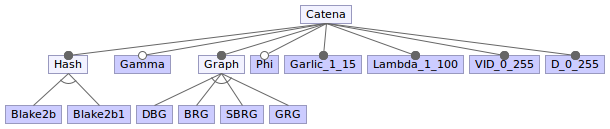
\includegraphics[width=0.8\textwidth]{images/Catena_Feature_model}
  \caption{Catena Feature Model.}
  \label{fm_catena}
\end{figure}


Project description
Project size in Classes and Functions
Project properties (SPL Model)
Features explained
Workload
Num Dimensions: 3b 5n\todo{3+2b 4n}
Whole configuration space: 3,145,728,000

Individual Feature Description (short):
\begin{description}
	\item [Hash] bal
	\item [Gamma] bla
	\item [Graph] bla
	\item [Phi] bla
	\item [Garlic] bla
	\item [Lambda] bla
	\item [VID] bla
	\item [D] bla
\end{description}

\subsection{H2}

\begin{figure}
  \centering
  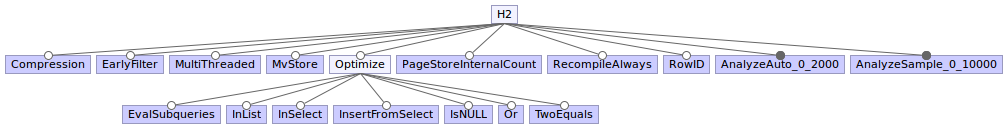
\includegraphics[width=0.8\textwidth]{images/H2_Feature_model}
  \caption{H2 Feature Model.}
  \label{fm_h2}
\end{figure}

Project description
Project size in Classes and Functions
Project properties (SPL Model)
Features explained
Workload
Num dimensions: 14b 2n
Whole configuration Space: 3,920,000,000


\begin{description}
	\item [Compression] bal
	\item [EarlyFilter] bla
	\item [MultiThreaded] bla
	\item [MvStore] bla
	\item [OptimizeEvalSubqueries] bla
	\item [OptimizeInList] bla
	\item [OptimizeInsertFromSelect] bla
	\item [OptimizeIsNull] bla
	\item [OptimizeOr] bla
	\item [PageStoreInternalCount] bla
	\item [RecompileAlways] bla
	\item [RowID] bla
	\item [AnalyzeAuto] bla
	\item [AnalyzeSample] bla
\end{description}

\subsection{Sunflow}

\begin{figure}
  \centering
  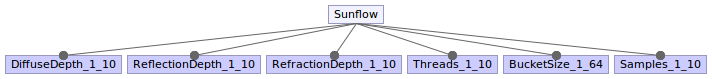
\includegraphics[width=0.8\textwidth]{images/Sunflow_Feature_model}
  \caption{Sunflow Feature Model.}
  \label{fm_sunflow}
\end{figure}

Project description
Project size in Classes and Functions
Project properties (SPL Model)
Features explained
Workload
Num dimensions: 6n
Whole configuration space: 6,400,000

\begin{description}
	\item [DiffuseDepth] bal
	\item [ReflectionDepth] bla
	\item [RefractionDepth] bla
	\item [Threads] bla
	\item [BucketSize] bla
	\item [Samples] bla
\end{description}


\section{Results}
\label{results}
% Present raw results:
External measurement impact

Configuration Sensitivity

Workload sensitivity

Performance-influence model accuracy of whole software execution

Performance- influence model accuracy on method level

% use quality metrics to describe
% Impact of configuration
% Impact of workload

\section{Discussion}
\label{discussion}

answer RQs

\section{Detailed Analysis}
\label{delailed_analysis}

concentrate on Interesting parts
with help of developed tools we want to

\subsection{GC Analysis}
\label{gc_analysis}

impact of GC (Java specific stuff)
GC on/off
GC with different settings

\subsection{Eclipse Plugin}
\label{eclipse_plugin}

Eclipse plugin structure and functionality (maybe example usecase - what is better with this tool in comparison to others)
discussion of usage scenarios

\subsection{FlameGraphs}
\label{flame_graph}

Flame graph overview / idea, intention, usage scenario
discussion of usage scenarios

\section{Threads on Validity}
\label{validity}
How meaningful are our Results

\subsection{Internal Validity}

Which methodes and analyse metrics
Probably other profiler (more precise)


\subsection{External Validity}

Which environment and wich subject systems
